\documentclass{article}
\usepackage[utf8]{inputenc}
\usepackage[english]{babel}
\usepackage[normalem]{ulem}
\usepackage{amssymb}
\usepackage{amsmath}
\usepackage{graphicx}
\usepackage{algorithm}
\usepackage{algorithmic}
\title{Rapport sur le projet d'Optimisation\\Support-Vector Machines}
\author{Kawisorn Kamtue \& Clémence Réda}
\date{\today}

\maketitle

\begin{document}

\section{Support Vector Machine}

Les \emph{Support Vector Machine solvers} (SVM) sont une catégorie d'algorithmes d'apprentissage statistique supervisé. Ils permettent de résoudre le problème de classification binaire suivant :\\

           
           Etant donnés $(x_i)_{i \leq m}$ des points dans $\mathbb{R}^n$, et $(y_i)_{i \leq m}$ les étiquettes des points tels que l'étiquette de $x_i$ soit $y_i \in \{-1, 1\}$, on cherche la droite qui sépare "le mieux possible" les points dans différentes classes, autrement dit, la frontière de Voronoi entre les deux classes.
           \begin{center}
           \begin{figure}[H]
           \centering
           \caption{Exemple de frontière pour deux classes : celles des points noirs et celle des points rouges}
           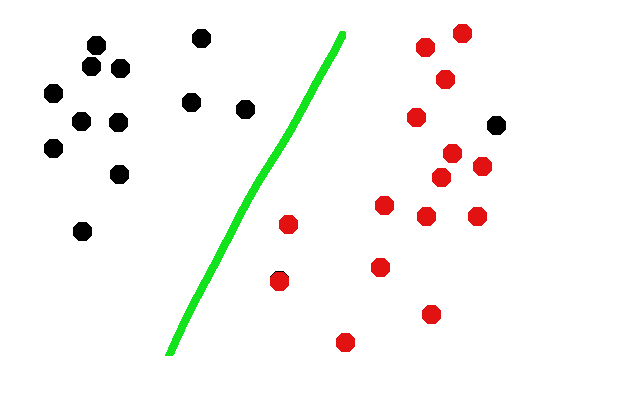
\includegraphics[scale=0.3]{images/voronoi.png}
           \end{figure}
           \end{center} 

\noidnent La frontière que l'on recherche est une fonction linéaire, donc de la forme (avec deux paramètres de dimension 1 $\omega$ et $b$) :\\

          \begin{center}
          $f : X \rightarrow \omega^{T}X + b$
          \end{center}

telle que :\\
 
         \begin{center}
         $\forall i, y_i = -1 \Rightarrow f(x_i) \leq -1$\\
         $\forall i, y_i = 1 \Rightarrow f(x_i) \geq 1$\\
         $\Leftrightarrow \forall i, y_i \times f(x_i) \geq 1$ (1)
         \end{center}

\newpage

Pour simplifier le problème, on peut prendre $\omega' =$ \begin{bmatrix}$\omega$\\ 1\end{bmatrix} (que l'on note par la suite $\omega$) pour supposer $b = 0$ sans perte de généralité.\\

Pour obtenir un résultat robuste, on souhaite que les deux droites $f(X) = 1$ et $f(X) = -1$ soient les plus distantes possibles. En effet, si ces deux droites sont trop proches, cela signifie que la probabilité d'erreur quant à la prédiction de la classe d'un point proche de ces droites sera importante.\\

La distance $\gamma$ entre ces deux droites se calcule de la façon suivante : soient $u, v$ deux points tels que $f(v) = 1$ et $f(u) = -1$. Alors :

      \begin{center}
      $\|f(v) - f(u)\| = \|\omega \times (v-u)\| = \|\omega\| \times \|(v-u)\| = \|\omega\| \times \|\gamma\| = \|1 - (-1)\| = 2$
      \end{center}

Finalement, le problème d'optimisation à résoudre pourrait être :\\
 
           \begin{centre}
           $max_{w}$ $\gamma = \frac{2}{\|w\|}$ avec (1)\\
           $\Leftrightarrow min_{w}$ $\|w\|$ avec (1)\\
           $\Leftrightarrow min_{w}$ $\frac{1}{2} \times \|w\|^2$ avec (1) pour faciliter les calculs
           \end{centre}

\bigskip

Un autre problème se pose si on s'arrête ici : par exemple, dans l'exemple de la frontière de Voronoi que l'on a vu ci-dessus, il n'existe pas de droite telle qu'il n'y ait que de points noirs d'un côté et que des points rouges de l'autre côté, ce qui contredit la condition (1). Le problème est alors infaisable. Pourtant, la droite dessinée en vert peut sembler acceptable comme frontière pour cet ensemble de points.\\

On tient compte de cette erreur en introduisant les variables $(z_i)_{i \leq m}$. Pour que la condition (1) soit toujours vérifiée, il faut que quand $y_i \times f(x_i) \geq 1$, $z_i = 0$ et lorsque $y_i \times f(x_i) < 1$, $z_i = 1 - y_i \times f(x_i)$. Le but étant de minimiser le nombre de ces erreurs, ie. points mal classés, on utilise un paramètre $C$ constant qui permet d'insister plus ou mins sur la minimisation de ces erreurs :\\ 


           \begin{centre}
           (P) $min_{w}$ $\frac{1}{2} \times \|w\| + C \times \sum_{i \leq m}z_i$\\
           avec $\forall i, z_i \geq 0$\\
           $\forall i, y_i \times (\omega^{T} x_i) \geq 1 - z_i$\\
           \end{centre}

\bigskip

Les fonctions que l'on a introduites sont toutes convexes. Si la dimension des points $(x_i)_i$ est petite, nous allons pouvoir utiliser la méthode de Newton pour résoudre ce problème. On verra par la suite le \emph{kernel trick} qui permettra de ne pas tenir compte de la dimension, mais seulement du nombre d'échantillons $(x_i)_i$.

\section{Calcul du dual}

Calculons le lagrangien du problème (P). Soit $\lambda$ le multiplicateur de Lagrange de dimension $1 \times m$:

              \begin{center}
              $\forall w, \lambda \in \mathbb{R}^{2m}, L(\omega, \lambda, z) = $\\
              $= \frac{1}{2} \|w\|^2 + C \times \sum_i z_i - \sum_i \lambda_i \times z_i$
              $+ \sum_i \lambda_i \times (1 - y_i \omega^{T} x_i)$\\
              $= \frac{1}{2} \|w\|^2 + C$\textbf{1}$^{T}z - C\lambda^{T}z + $\textbf{1}$^{T}\lambda - \sum_i \lambda_i \times y_i \omega^{T} x_i$\\
              $= \frac{1}{2} (\|w - \sum_i \lambda_iy_ix_i\|^2_2 - \|\sum_i \lambda_iy_ix_i\|^2_2)$
              $+ (C$\textbf{1}$ - \lambda)^{T}z + $\textbf{1}$^{T}\lambda$\\
              \end{center}

Minimisons L par rapport à $\omega$. Comme le langrangien est convexe en $\omega$, il faut annuler le gradient :\\

              \begin{center}
              $\nabla_{\omega} L(\omega, \lambda, z) = \frac{1}{2}(2\omega - 2\sum_i \lambda_iy_ix_i) + 0 = 0$\\
              $\Leftrightarrow \omega = \sum_i \lambda_iy_ix_i$ (1)\\
              \end{center}

Minimisons L par rapport à $z$. Comme le langrangien est convexe en $z$, il faut annuler le gradient :\\

              \begin{center}
              $\nabla_{z} L(\omega, \lambda, z) = 0 + C$\textbf{1}\textbf{$1_{z>0}$}$^T - \lambda$\textbf{$1_{z>0}$}$^T = 0$\\
              $\Leftrightarrow mC - \sum_i \lambda_i = 0$ si $z_i > 0$\\
              $\Leftrightarrow mC = \sum_i \lambda_i$ si $z_i > 0$ (2)\\
              \end{center}

Le minimum en L par rapport à $z$ a une valeur finie ssi $C$\textbf{1}$ - \lambda = 0$. On obtient le problème dual en injectant les valeurs de $\omega$ et de $z$ dans le lagrangien :\\

             \begin{center}
             $max_{\lambda \in \mathbb{R}^{+m}} -\frac{1}{2}\|\sum_i\lambda_iy_ix_i\|^2_2 + $\textbf{1}$^T\lambda$ par (1)\\ 
             avec $\forall i, 0 \leq \lambda_i \leq C$ si $z_i > 0$ (vient de (2))\\
             \end{center}

On obtient la solution optimale du primal $(\omega^*, z^*)$ à partir de celle du dual $\lambda^*$ :

             \begin{center}
             (1) $\omega^{*} = \sum_i \lambda^{*}_i y_i x_i$
             \end{center}

\section{Utilisation de l'astuce du noyau (\emph{kernel trick})}

Pour pouvoir trouver efficacement la solution au problème avec la méthode de Newton, il faut s'affranchir de la contrainte quadratique sur la dimension des échantillons. On note X la matrice des échantillons, et la matrice du noyau $K = X^TX$, avec $K \geq 0$. On montre alors que le problème dual peut se réécrire de la façon suivante :\\

                 \begin{center}
                 $max$ $-\frac{1}{2}\lambda^Tdiag(y)Kdiag(y)\lambda+$\textbf{1}$^T\lambda$\\
                 avec $\forall i, 0 \leq \lambda_i \leq C$ 
                 \end{center}

On remarque que la dimension $m$ des échantillons n'intervient plus, et que donc la complexité de la résolution du problème ne dépend que du nombre d'échantillons. 

\section{Méthode de la barrière logarithmique}

Enfin, on peut s'affranchir des contraintes d'inégalité sur le multiplicateur de Lagrange $\lambda$ en posant la fonction barière suivante :\\

          \begin{center}
          $\Phi(\lambda) = \sum_i (- log(C - \lambda_i) - log(\lambda_i)) = \sum_i log(\frac{1}{(C - \lambda_i)\lambda_i})$ 
          \end{center}

Le problème à optimiser devient alors :\\

          \begin{center}
          $max$ $-\frac{1}{2}\lambda^Tdiag(y)Kdiag(y)\lambda+$\textbf{1}$^T\lambda + \Phi(\lambda)$\\ 
          \end{center}

\section{Résultats}

\end{document}
